\documentclass[xcolor=dvipsnames, 10pt]{beamer}
\usepackage{textpos}
\usepackage{amsmath}
\usepackage{graphicx} 
\usepackage[com pat = 1.1.0]{tikz-feynman}
\usepackage{multirow}
\usepackage[utf8]{inputenc}
\usepackage{color, colortbl}
\usepackage{relsize}
\usepackage{slashed}
\usepackage[many]{tcolorbox}

%%% ====================================================================
% from cms-tdr.cls 
% PENNAMES
\usepackage[low-sup]{subdepth}  
% corrects normal super/sub after subdepth: 
% https://tex.stackexchange.com/questions/352936/wrong-superscript-placement-with-hepparticles
% \usepackage[italic,italicGreek]{heppennames2}
\usepackage[pazoGreek]{heppennames2}
\usepackage{ptdr-definitions}
%%% ====================================================================



\usetheme{Madrid}
\useinnertheme{rectangles}

% set bib
\setbeamertemplate{bibliography item}{\insertbiblabel}
\setbeamertemplate{bibliography entry title}{}
\setbeamertemplate{bibliography entry location}{}
\setbeamertemplate{bibliography entry note}{}

% NWU color theme
% \usecolortheme{whale}
\definecolor{NUpurple}{RGB}{078,042,132}
\definecolor{NUpurple60}{RGB}{131,110,170}
\definecolor{NUpurple30}{RGB}{182,172,209}
\definecolor{NUpurple10}{RGB}{228,224,238}
\definecolor{Gray}{gray}{0.9}
\usecolortheme[named=NUpurple]{structure}
\setbeamercolor{block title}{bg=NUpurple}

% NWU CMS Logo
\addtobeamertemplate{frametitle}{}{
    \begin{textblock*}{\textwidth}(.9\textwidth,-0.75cm)
    
\includegraphics[width=0.05\textwidth]{slides/logos/logo_nwu.png}
    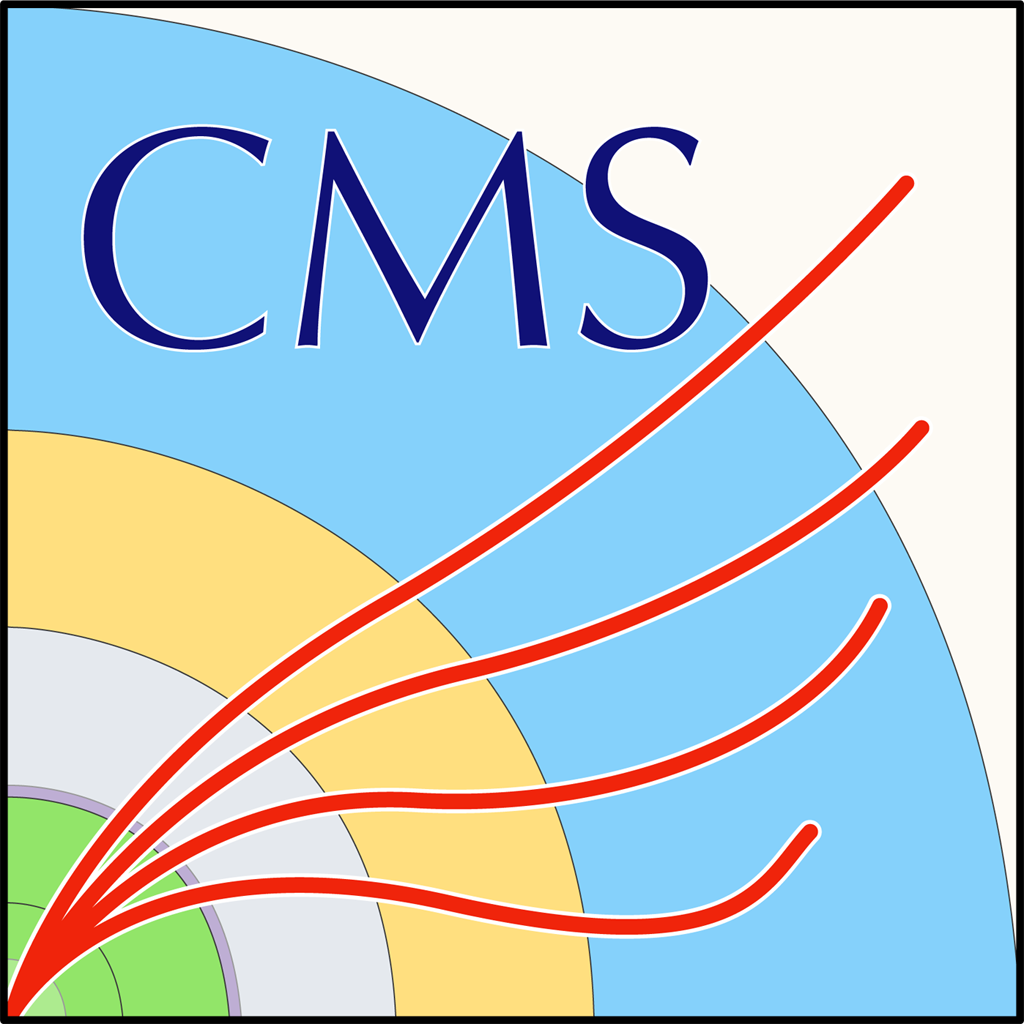
\includegraphics[width=0.05\textwidth]{slides/logos/logo_cms.png}
    \end{textblock*}}
    

% extra beamer settings
\AtBeginSection[]{\begin{frame}{Table of Contents}\setcounter{tocdepth}{2}\tableofcontents[currentsection, hideothersubsections]\end{frame}}



\title[\BWl measurement]{Measurement of W boson Branching Fraction in p-p Collisions at $\sqrt{s} = 13\TeV$  with the CMS Experiment}
\date{\today}
\author[Z. Chen]{Ziheng Chen}
\institute[NWU]{Department of Physics and Astronomy, \\ Northwestern University}
% \logo { 
\includegraphics[width=0.1\textwidth]{slides/logos/logo_nwu.png} \qquad 
% 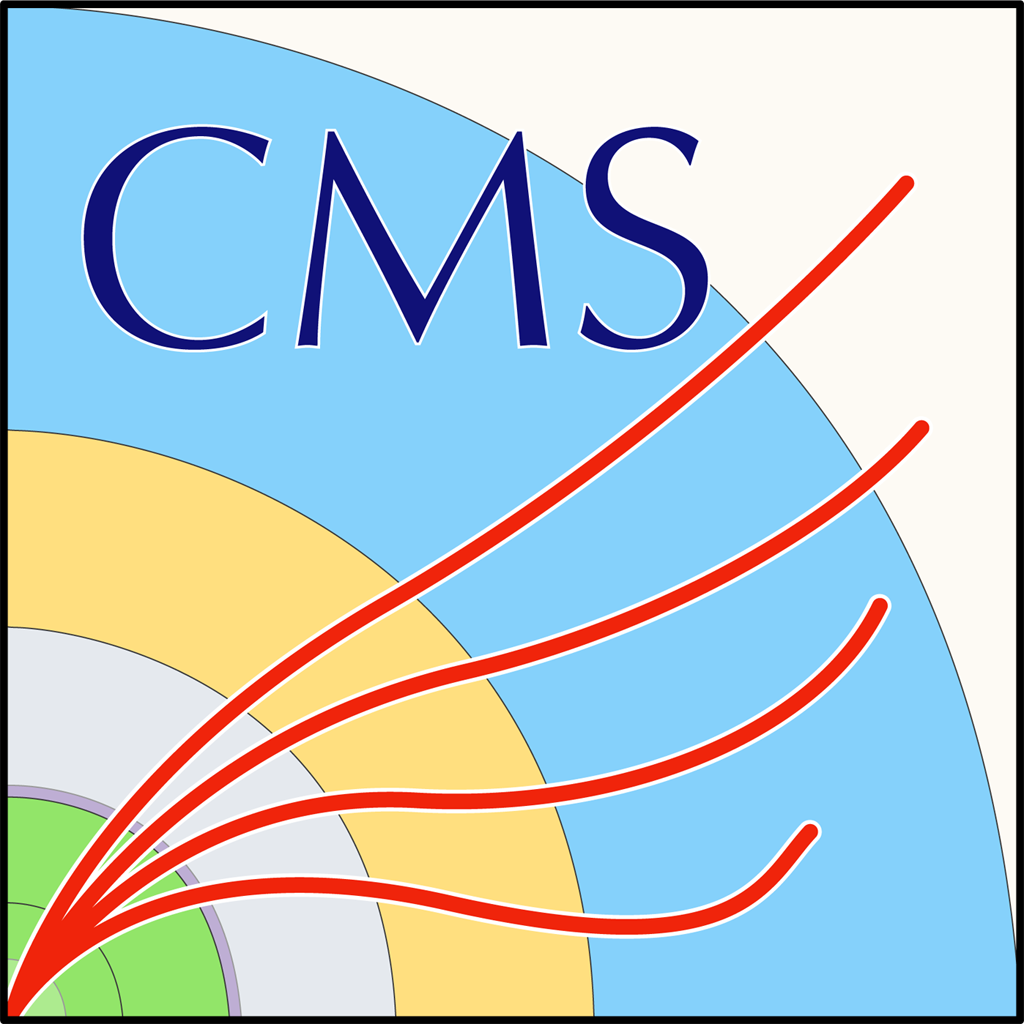
\includegraphics[width=0.1\textwidth]{slides/logos/logo_cms.png}}

\addtobeamertemplate{title page}
{\centering \footnotesize {\color{NUpurple} Defence for the Ph.D. Degree in the Field of Physics  \rule{\linewidth}{0.2mm}} } 
{\centering \footnotesize \begin{center}  supervisor: Prof. Mayda Velasco  \end{center} }

    
\begin{document}
% title page
\begin{frame}{} \titlepage \end{frame}
% contents page
\begin{frame}{Table of Contents}\setcounter{tocdepth}{2}\tableofcontents \end{frame}
% sections
\section{Introduction}

% -------------
% new frame
% -------------
\begin{frame}{Introduction}
\smaller
    
    \begin{columns}
        \column{0.5\textwidth}
        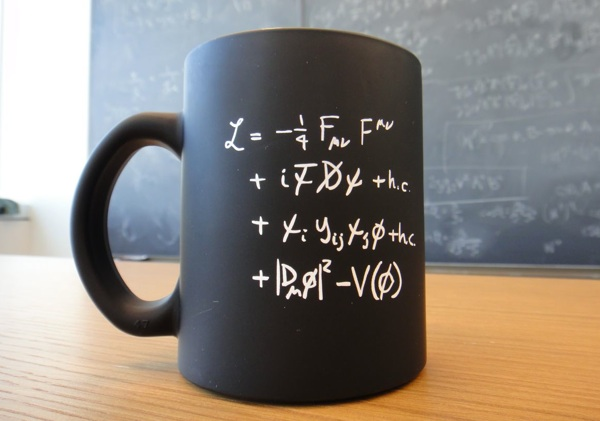
\includegraphics[width=\textwidth]{slides/figures/cernmug.jpeg}
        \column{0.5\textwidth}
        \begin{itemize} 
            \item The Standard Model (SM) represents the our current best understanding of the matter and force.
            \item It includes three generations of leptons (\Pe\PGne), (\PGm\PGnGm), (\PGt\PGnGt) and quarks (\PQu\PQd), (\PQc\PQs), (\PQt\PQb) as matter paticles, four gauge bosons \PGg, \PW, \PZ, \Pg as force particles, and one Higgs boson to generate mass.
            \item SM has been very successful in explaining and predicting experimental observations so far.
        \end{itemize}
    \end{columns}
    
    \vspace{0.05\textheight}
    \begin{itemize}
        \item The interaction between the leptons and \PW boson is encapsulated in the term $i\bar{\psi}\slashed{D}\psi$:
        \begin{equation*} \tiny
            i\bar{\psi}\slashed{D}\psi = 
            \bar{\chi}_L \gamma^\mu \big( i \partial_\mu  - \textcolor{red}{g} \frac{\tau_a}{2} W^a_\mu  -g'\frac{Y}{2} B_\mu \big) \chi_L 
            + \bar{\psi}_R \gamma^\mu \big( i \partial_\mu -g'\frac{Y}{2} B_\mu \big) \psi_R 
            - g_s (\bar{q}\gamma^\mu  T_{a} q) G_\mu^a 
        \end{equation*}
    \end{itemize}
\end{frame}



% -------------
% new frame
% -------------
\begin{frame}{Introduction}
\smaller 
    
    \begin{center}
    \resizebox{0.6\textwidth}{!}{    \feynmandiagram [inline=(d.base), small, horizontal=d to b] {
        a[particle=\PGne] -- [fermion] b [dot] -- [fermion] c[particle=\Pe], 
        b -- [boson, edge label=\PW] d,}; 
    = \qquad
    \feynmandiagram [inline=(d.base), small, horizontal=d to b] {
        a[particle=\PGnGm] -- [fermion] b [dot] -- [fermion] c[particle=\PGm],
        b -- [boson, edge label=\PW] d, }; 
    = \qquad
    \feynmandiagram [inline=(d.base), small, horizontal=d to b] {
        a[particle=\PGnGt] -- [fermion] b [dot] -- [fermion] c[particle=\PGt],
        b -- [boson, edge label=\PW] d,};}
    \end{center}
    
    \vspace{0.05\textheight}
    \begin{itemize} 
        \item One of the essential assumptions in SM is that the coupling strength $g$ is the same for all three generations of leptons, $g_\Pe = g_\PGm = g_\PGt \equiv g $, known as Lepton Universality (LU) in the weak interaction.
        \item Tests of the SM LU can be performed by studies of the leptonic decays of \PW bosons.
        \item In high-energy regime, the tests of lepton universality related to \PW boson have been performed on colliders.
        \begin{itemize} 
        \smaller 
            \item SPS and Tevatron using $\Pp\bar{\Pp}\to \PW$.
            \item LEP using $\Pe\bar{\Pe}\to \PW \PW$.
            \item LHC using $\Pp\Pp \to \PW$ and $\Pp\Pp \to \ttbar \to \PQb\PW \PAQb\PW$.
        \end{itemize}
        \item In low-energy regime, some of the most stringent LU tests come from the charge weak decays of mesons (e.g. \PD, \PB) and leptonic decays of taus~\cite{Amhis:2019ckw}. While most show high precision agreement with LU, tensions have been recently observed in the semileptonic decays of \PB mesons by Belle~\cite{Huschle:2015rga, Sato:2016svk, Hirose:2016wfn}, BaBar ~\cite{Lees:2012xj, Lees:2013uzd} and LHCb~\cite{Aaij:2015yra,Aaij:2017uff, Aaij:2017deq}.
    \end{itemize}
\end{frame}



% -------------
% new frame
% -------------
\begin{frame}{}
\smaller
    
    \begin{block}{SPS and Tevatron}
        \begin{columns}
            % add column
            \column{0.65\textwidth}
            \begin{itemize}
                \item the $\sigma_{\Pp\bar{\Pp}\to \PW} \times \BWl$ in three leptonic channels were measured by UA1~\cite{Albajar:1988ka}, UA2~\cite{appel1986measurement, Alitti:1991eh, Alitti:1992hv}, CDF~\cite{Abe:1990sd, Abe:1992ys, Abe:1991fb}, D0~\cite{Abbott:1999tt, Abazov:2003sv, Abachi:1995xc, Abbott:1999pk}.
                \item taus were reconstructed in the hadronic decay modes.
                \item Combined average $g^\PW_\PGt / g^\PW_\Pe = 0.988\pm 0.025$ were determined by \DZERO~\cite{Abbott:1999pk} consistent with SM.  
            \end{itemize}
            
            % add column
            \column{0.3\textwidth}
            \centering
            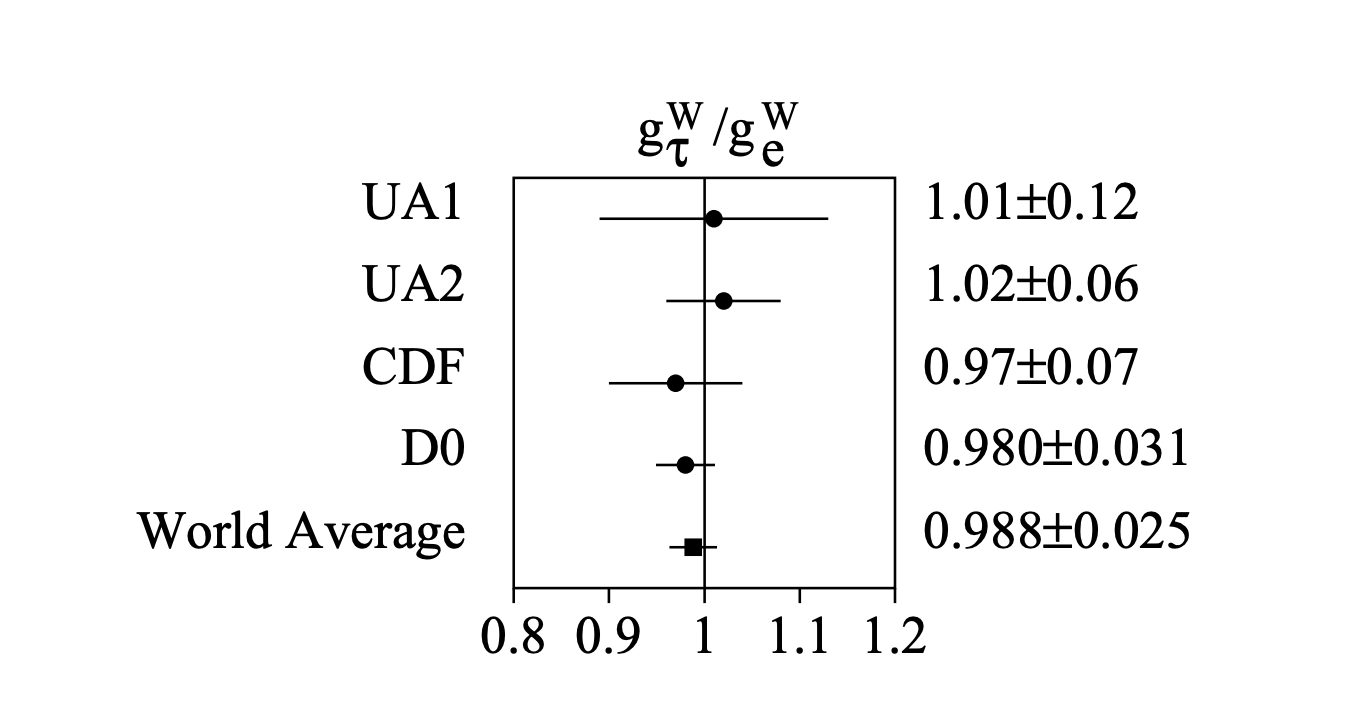
\includegraphics[width=\textwidth]{chapters/Introduction/sectionRelatedWorks/figures/spsTevatron.png}
        \end{columns}
    \end{block}
    
    \begin{block}{LEP-II}
        \begin{columns}
            % add column
            \column{0.65\textwidth}
            \begin{itemize}
                \item three individual leptonic \BWl were measured using pair-produced \WW from the electron-position collision by OPAL~\cite{Abbiendi:2007rs}, DELPHI~\cite{Abdallah:2003zm}, L3~\cite{Achard:2004zw}, ALEPH~\cite{Heister:2004wr}.
                \item the most precise and the only \BWl measurement available in PDG~\cite{pdg2020}.
                \item The LEP combined result~\cite{Schael:2013ita} showed agreement between electron and muon channel agree with each other, but tau channel was $2.6 \; \sigma$ above the average $$ \tiny 2\BWt/ \BWem = 1.066 \pm 0.025 $$ comparing with the SM prediction 0.999~\cite{Denner:1991kt,Rtau,dEnterria:2016rbf}.
            \end{itemize}
            
            % add column
            \column{0.3\textwidth}
            \centering
            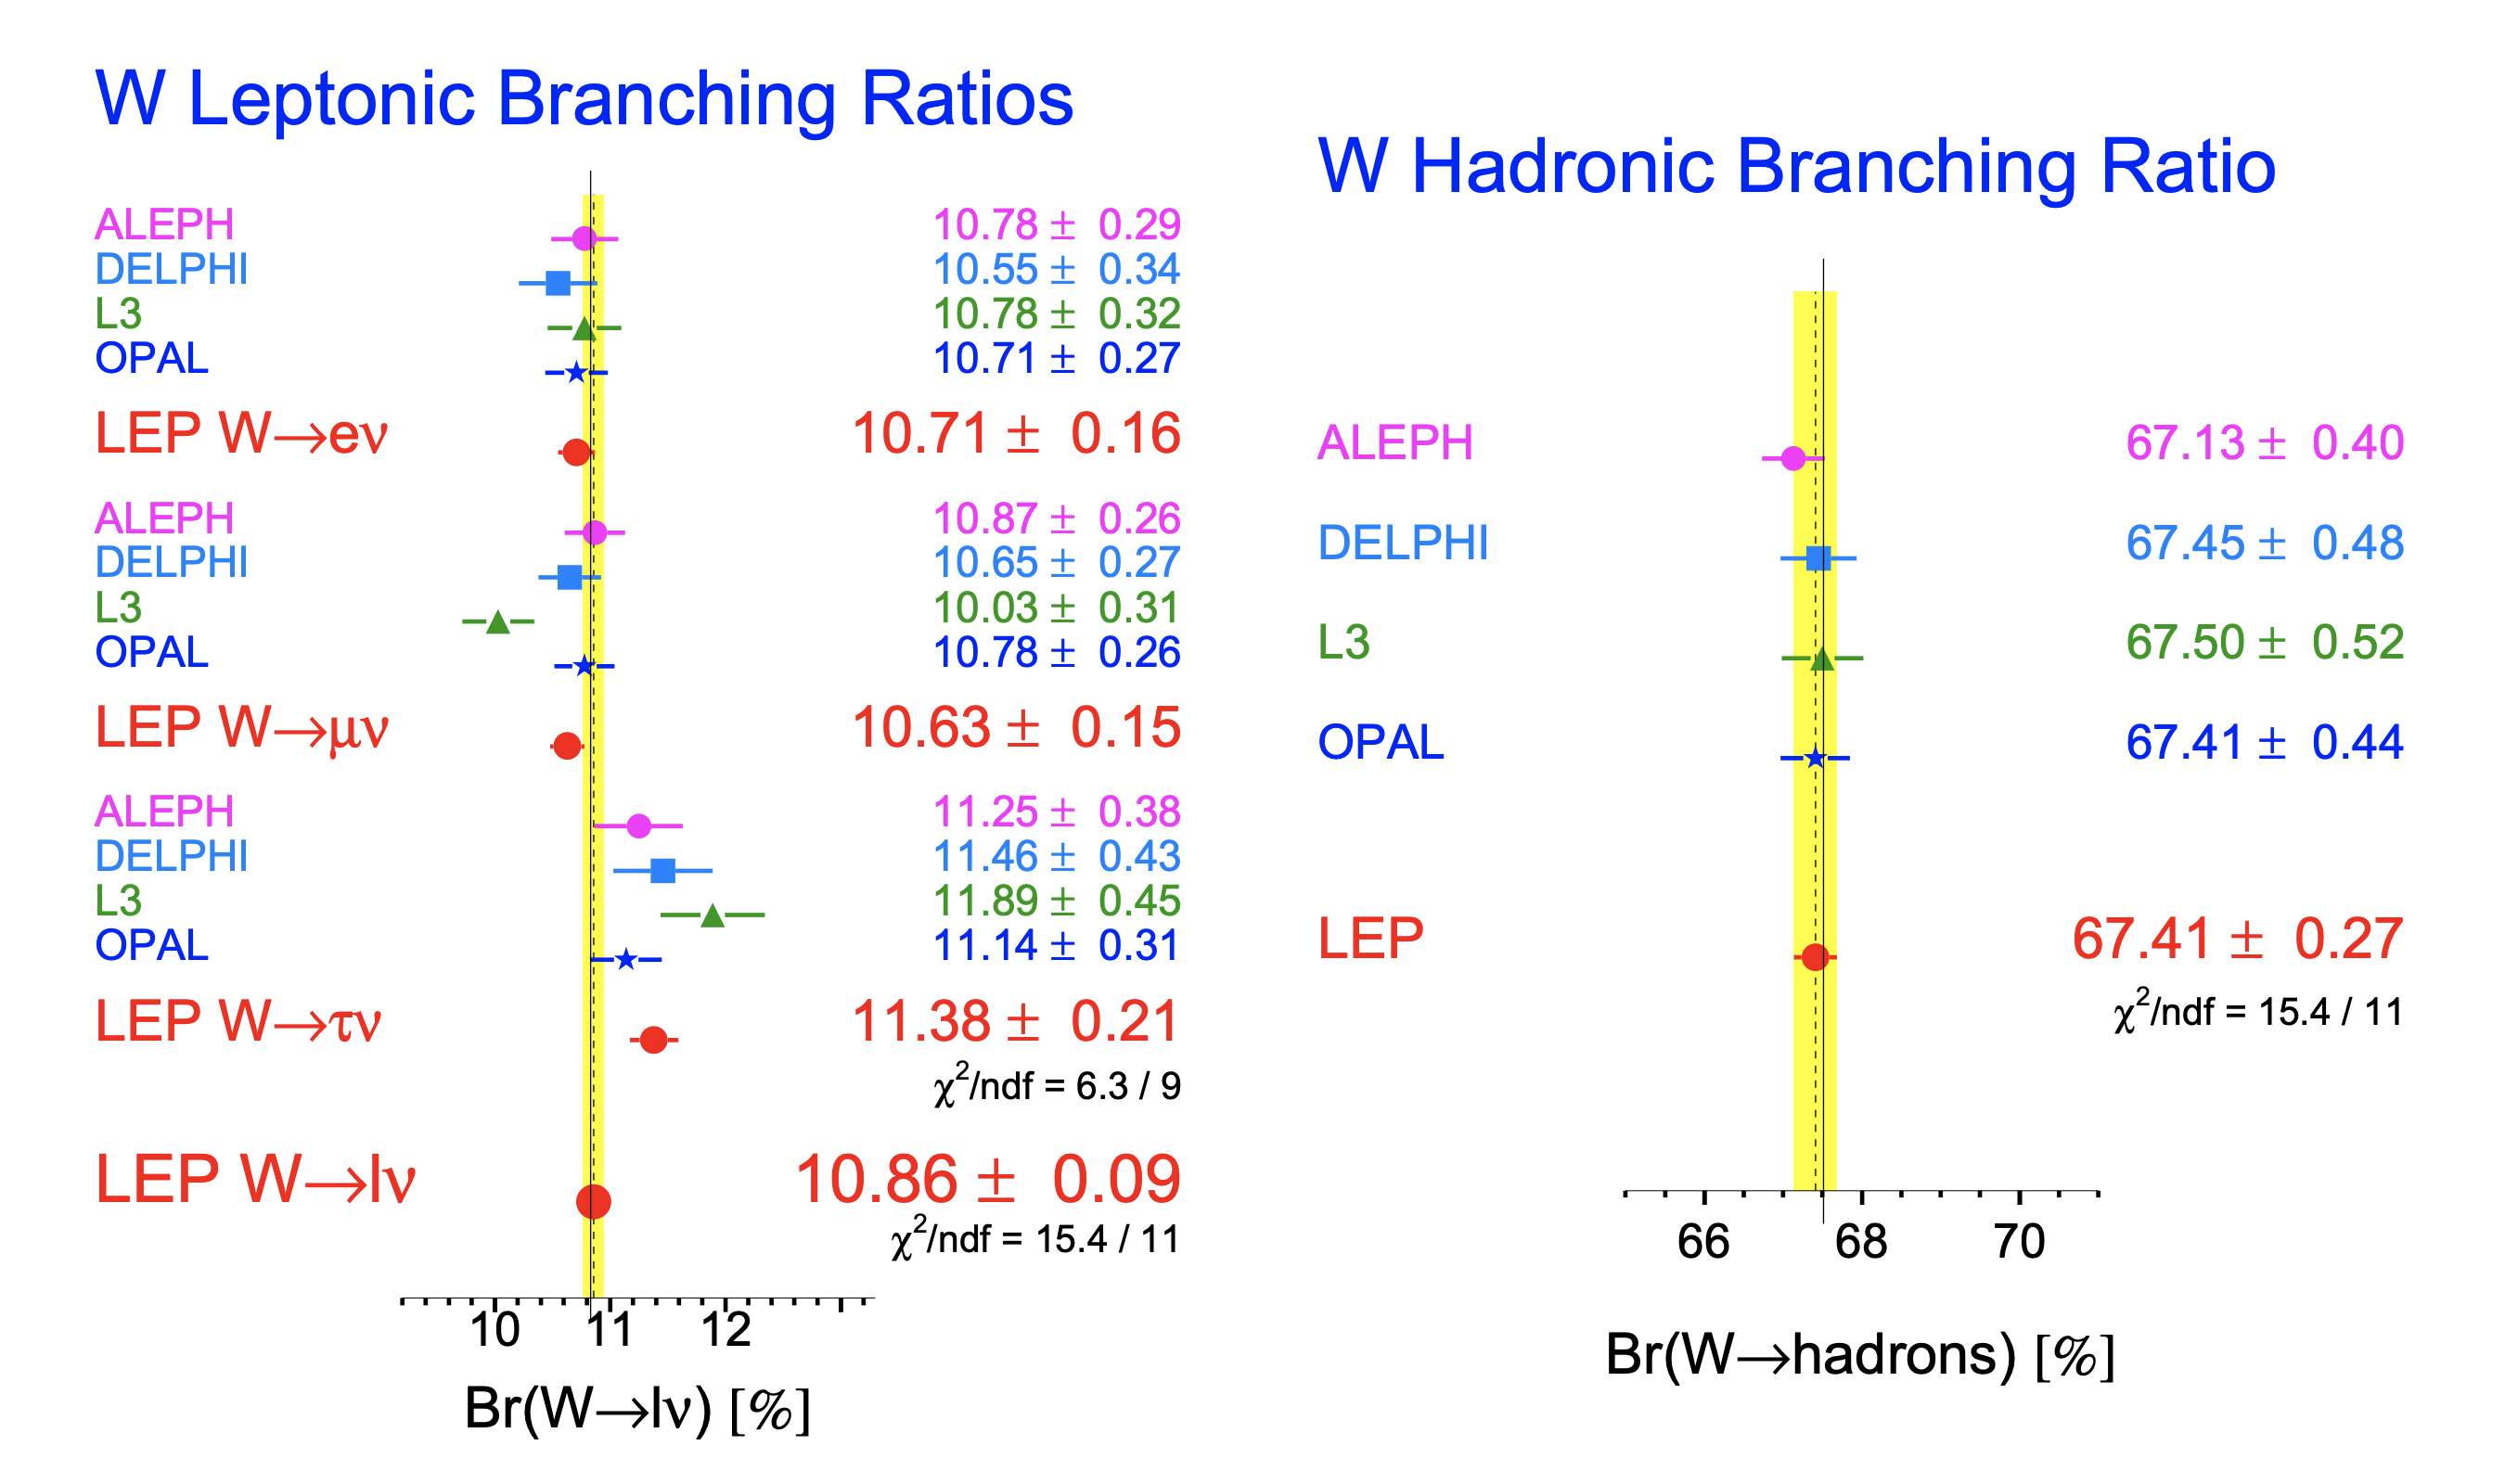
\includegraphics[width=\textwidth, trim=0 0 25cm 0, clip]{chapters/Introduction/sectionRelatedWorks/figures/lep.png}
        \end{columns}
    \end{block}
\end{frame}





% -------------
% new frame
% -------------
\begin{frame}{}
\smaller
    
    \begin{block}{LHC run-1}
        In the LHC run-1 at $\sqrt{s}=$ 7\TeV and 8\TeV, the LU between $\PW \to \Pe \PGn$ and $\PW \to \PGm \PGn$ has been tested by ATLAS~\cite{Aaboud:2016btc} and LHCb~\cite{Aaij:2015zlq, Aaij:2016qqz}.
        \begin{itemize}
            \item the \wjets cross-section was measured in electron and muon channels, ratio of which leads to $\BWm/\BWe$ as 1.003(10) by ATLAS and 0.980(18) by LHCb.
            \item the results agree with SM lepton universality.
        \end{itemize}
    \end{block}
                
   \begin{block}{LHC run-2}
        \begin{columns}[c]
            % add column
            \column{0.65\textwidth}           
            In the LHC run-2 at $\sqrt{s}=$ 13\TeV, ATLAS~\cite{Aad:2020ayz} has most recently published a test between muon and tau.
            \begin{itemize}
                \item use $\Pp\Pp\to\ttbar\to\PQb\PW\PAQb\PW$ events selected with \cmm, \cem plus two \PQb tagged jets final states.
                \item tau leptons are probed via muons from $\PGt\to\PGm\PAGnGm\PGnGt$, which tend to be softer and more displaced than prompt muons.
                \item fitting the transverse displacement and \pt of the probing muon leads to the ratio $$ \tiny \BWt/\BWm = 0.992 \pm 0.013 $$ consistent with the LU.
            \end{itemize}
            
            % add column
            \column{0.3\textwidth}
            \centering
            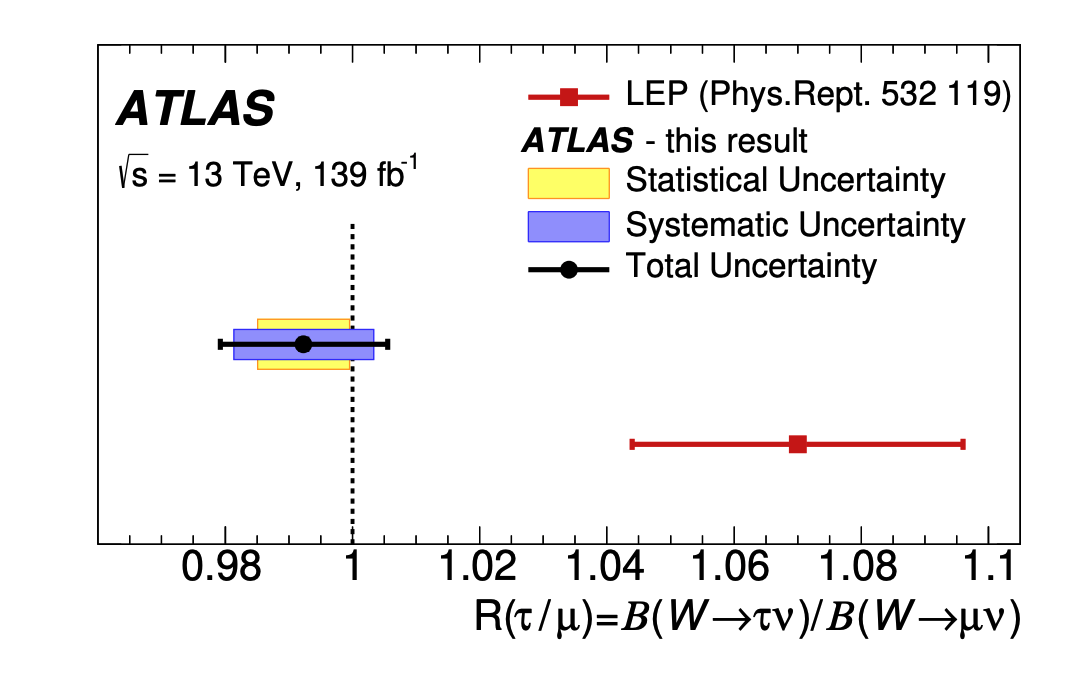
\includegraphics[width=\textwidth]{chapters/Introduction/sectionRelatedWorks/figures/atlas.png}
        \end{columns}
    \end{block}
\end{frame}






% -------------
% new frame
% -------------
\begin{frame}{}
\smaller
    \begin{columns}
        % add column
        \column{0.55\textwidth}
        \begin{block}{}
            \centering
            \small{\ttbar} process
            \resizebox{0.98\textwidth}{!}{    \feynmandiagram[small,horizontal=a to b]{
        i1 [particle=\PQq] -- [fermion] a -- [fermion] i2 [particle=\PQq],
        a -- [gluon, edge label=\Pg] b,
        f1 [particle=\PQt] -- [fermion] b -- [fermion] f2 [particle=\PQt],
        % top decay
        f1b[particle=\PQb] -- [fermion] f1 -- [photon] f1W [particle=\PW, red],
        f2b[particle=\PQb] -- [anti fermion] f2 -- [photon] f2W [particle=\PW, red],
        f1 -- [opacity=0.0] f2,
        f1W -- [opacity=0.0] f2W,
        f1b -- [opacity=0.0] f1W,
        f2b -- [opacity=0.0] f2W,
    }; \qquad
    \feynmandiagram[small,horizontal=a to b]{
        i1 [particle=\Pg] -- [gluon] a -- [gluon] i2 [particle=\Pg],
        a -- [gluon, edge label=\Pg] b,
        f1 [particle=\PQt] -- [fermion] b -- [fermion] f2 [particle=\PQt],
        % top decay
        f1b[particle=\PQb] -- [fermion] f1 -- [photon] f1W [particle=\PW, red],
        f2b[particle=\PQb] -- [anti fermion] f2 -- [photon] f2W [particle=\PW, red],
        f1 -- [opacity=0.0] f2,
        f1W -- [opacity=0.0] f2W,
        f1b -- [opacity=0.0] f1W,
        f2b -- [opacity=0.0] f2W,
    }; \qquad
    \feynmandiagram[small, vertical=a to b, horizontal=a to f1]{
        i1 [particle=\Pg] -- [gluon] a -- [anti fermion] f1 [particle=\PQt],
        a -- [fermion, edge label=\PQt] b,
        i2 [particle=\Pg] -- [gluon] b -- [fermion] f2 [particle=\PQt],
        % top decay
        f1b[particle=\PQb] -- [fermion] f1 -- [photon] f1W [particle=\PW, red],
        f2b[particle=\PQb] -- [anti fermion] f2 -- [photon] f2W [particle=\PW, red],
        f1 -- [opacity=0.0] f2,
        f1W -- [opacity=0.0] f2W,
        f1b -- [opacity=0.0] f1W,
        f2b -- [opacity=0.0] f2W,
        % i1 -- [opacity=0.0] i2,
        % f1 -- [opacity=0.0] f2,
    };}
        \end{block}
        % add column
        \column{0.4\textwidth}
        \begin{block}{}
            \centering
            \small{\tW} process
            \resizebox{0.98\textwidth}{!}{    \feynmandiagram[scale=0.7][horizontal=a to b]{
        i1 [particle=\PQb] -- [fermion] a -- [gluon] i2 [particle=\Pg],
        a -- [fermion, edge label=\PQb] b,
        f1 [particle=\PW , red] -- [photon] b -- [fermion] f2 [particle=\PQt],
        f2b[particle=\PQb] -- [anti fermion] f2 -- [photon] f2W [particle=\PW, red],
        f1 -- [opacity=0.0] f2W,
    }; \qquad
    \feynmandiagram[scale=0.7][vertical=a to b]{
        i1 [particle=\PQb] -- [fermion] a -- [photon] f1 [particle=\PW, red],
        a -- [fermion, edge label=\PQb] b,
        i2 [particle=\Pg] -- [gluon] b -- [fermion] f2 [particle=\PQt],
        f2b[particle=\PQb] -- [anti fermion] f2 -- [photon] f2W [particle=\PW, red],
        i1 -- [opacity=0.0] i2,
        f1 -- [opacity=0.0] f2W -- [opacity=0.0] f2b,
    };}
        \end{block}
    \end{columns}
    
    \vspace{0.1\textheight}
    \begin{itemize}
        \item This analysis presents a CMS measurement of three individual \BWl and a test of lepton universality in the \PW decay, 
        \begin{itemize} 
        \smaller
            \item use the run 2016 dataset from the LHC $\sqrt{s}=13\TeV$ proton-proton collisions.
            \item treat \ttbar and \tW processes as the primary signals.
        \end{itemize}       
        \item Motivations
        \begin{itemize} 
        \smaller
            \item The measurements of three \PW leptonic branching fractions have not been improved for more than a decay since LEP;
            \item LEP's $R_{\PGt/(e,\PGm)}$ shows a $2.6\,\sigma$ deviation from the SM prediction.
        \end{itemize}
        \item Opportunities
        \begin{itemize} 
        \smaller
            \item LHC 13\TeV \Pp-\Pp collisions produce a large number of \ttbar events giving $\PW\PW$ pairs;
            \item The improved \PQb tagging allows to select \ttbar events with a high purity;
            \item The improved \PGth identification enables to efficiently select \PW tauonic decays.
        \end{itemize}
    \end{itemize}
\end{frame}
    
    
    
    
    
% \begin{frame}{Introduction}
%     \begin{center}
%     \begin{itemize} \smaller
%         \item A
%         \item B
%     \end{itemize}
%     \end{center}
    
%     \begin{center}
%     \begin{columns}
%         % add column
%         \column{0.4\textwidth}
%         add column
        
%         % add column
%         \column{0.6\textwidth}
%         add column
%     \end{columns}
%     \end{center}
% \end{frame}
    

            

        


% \section{The CMS and Tau Reconstruction}
\begin{frame}{CMS Detector}
    \begin{center}
        \includegraphics[width=0.9\textwidth]{chapters/CMSExperiment/sectionDetector/figures/cmsDetector.png}
    \end{center}
\end{frame}



%

\begin{frame}{}
\smaller
    \begin{columns}
    \column{0.6\textwidth}

    \begin{itemize} 
        \item Brain of the detector: Two-level trigger system.
        \item level-1 trigger (L1T)
        \begin{itemize} 
            \item customized ASICs and onsite FPGAs
            \item consider muon chamber and calorimeter
            \item 40MHz to 100kHz
            \item comprised of local, regional and global 
            \item latency budget 4\mus 
        \end{itemize}
        
        \item high-level trigger (HLT)
        \begin{itemize} 
            \item CPU. commodity computers of builder-filter.
            \item run a streamlined version of offline reconstruction software, filter with a HLT menu
            \item 100\;kHz to 1\;kHz
            \item in 2012, 13000 CPU cores 200 ms/event \cite{Trocino:2014jya}
        \end{itemize}
    \end{itemize}
    
    
    \column{0.4\textwidth}
    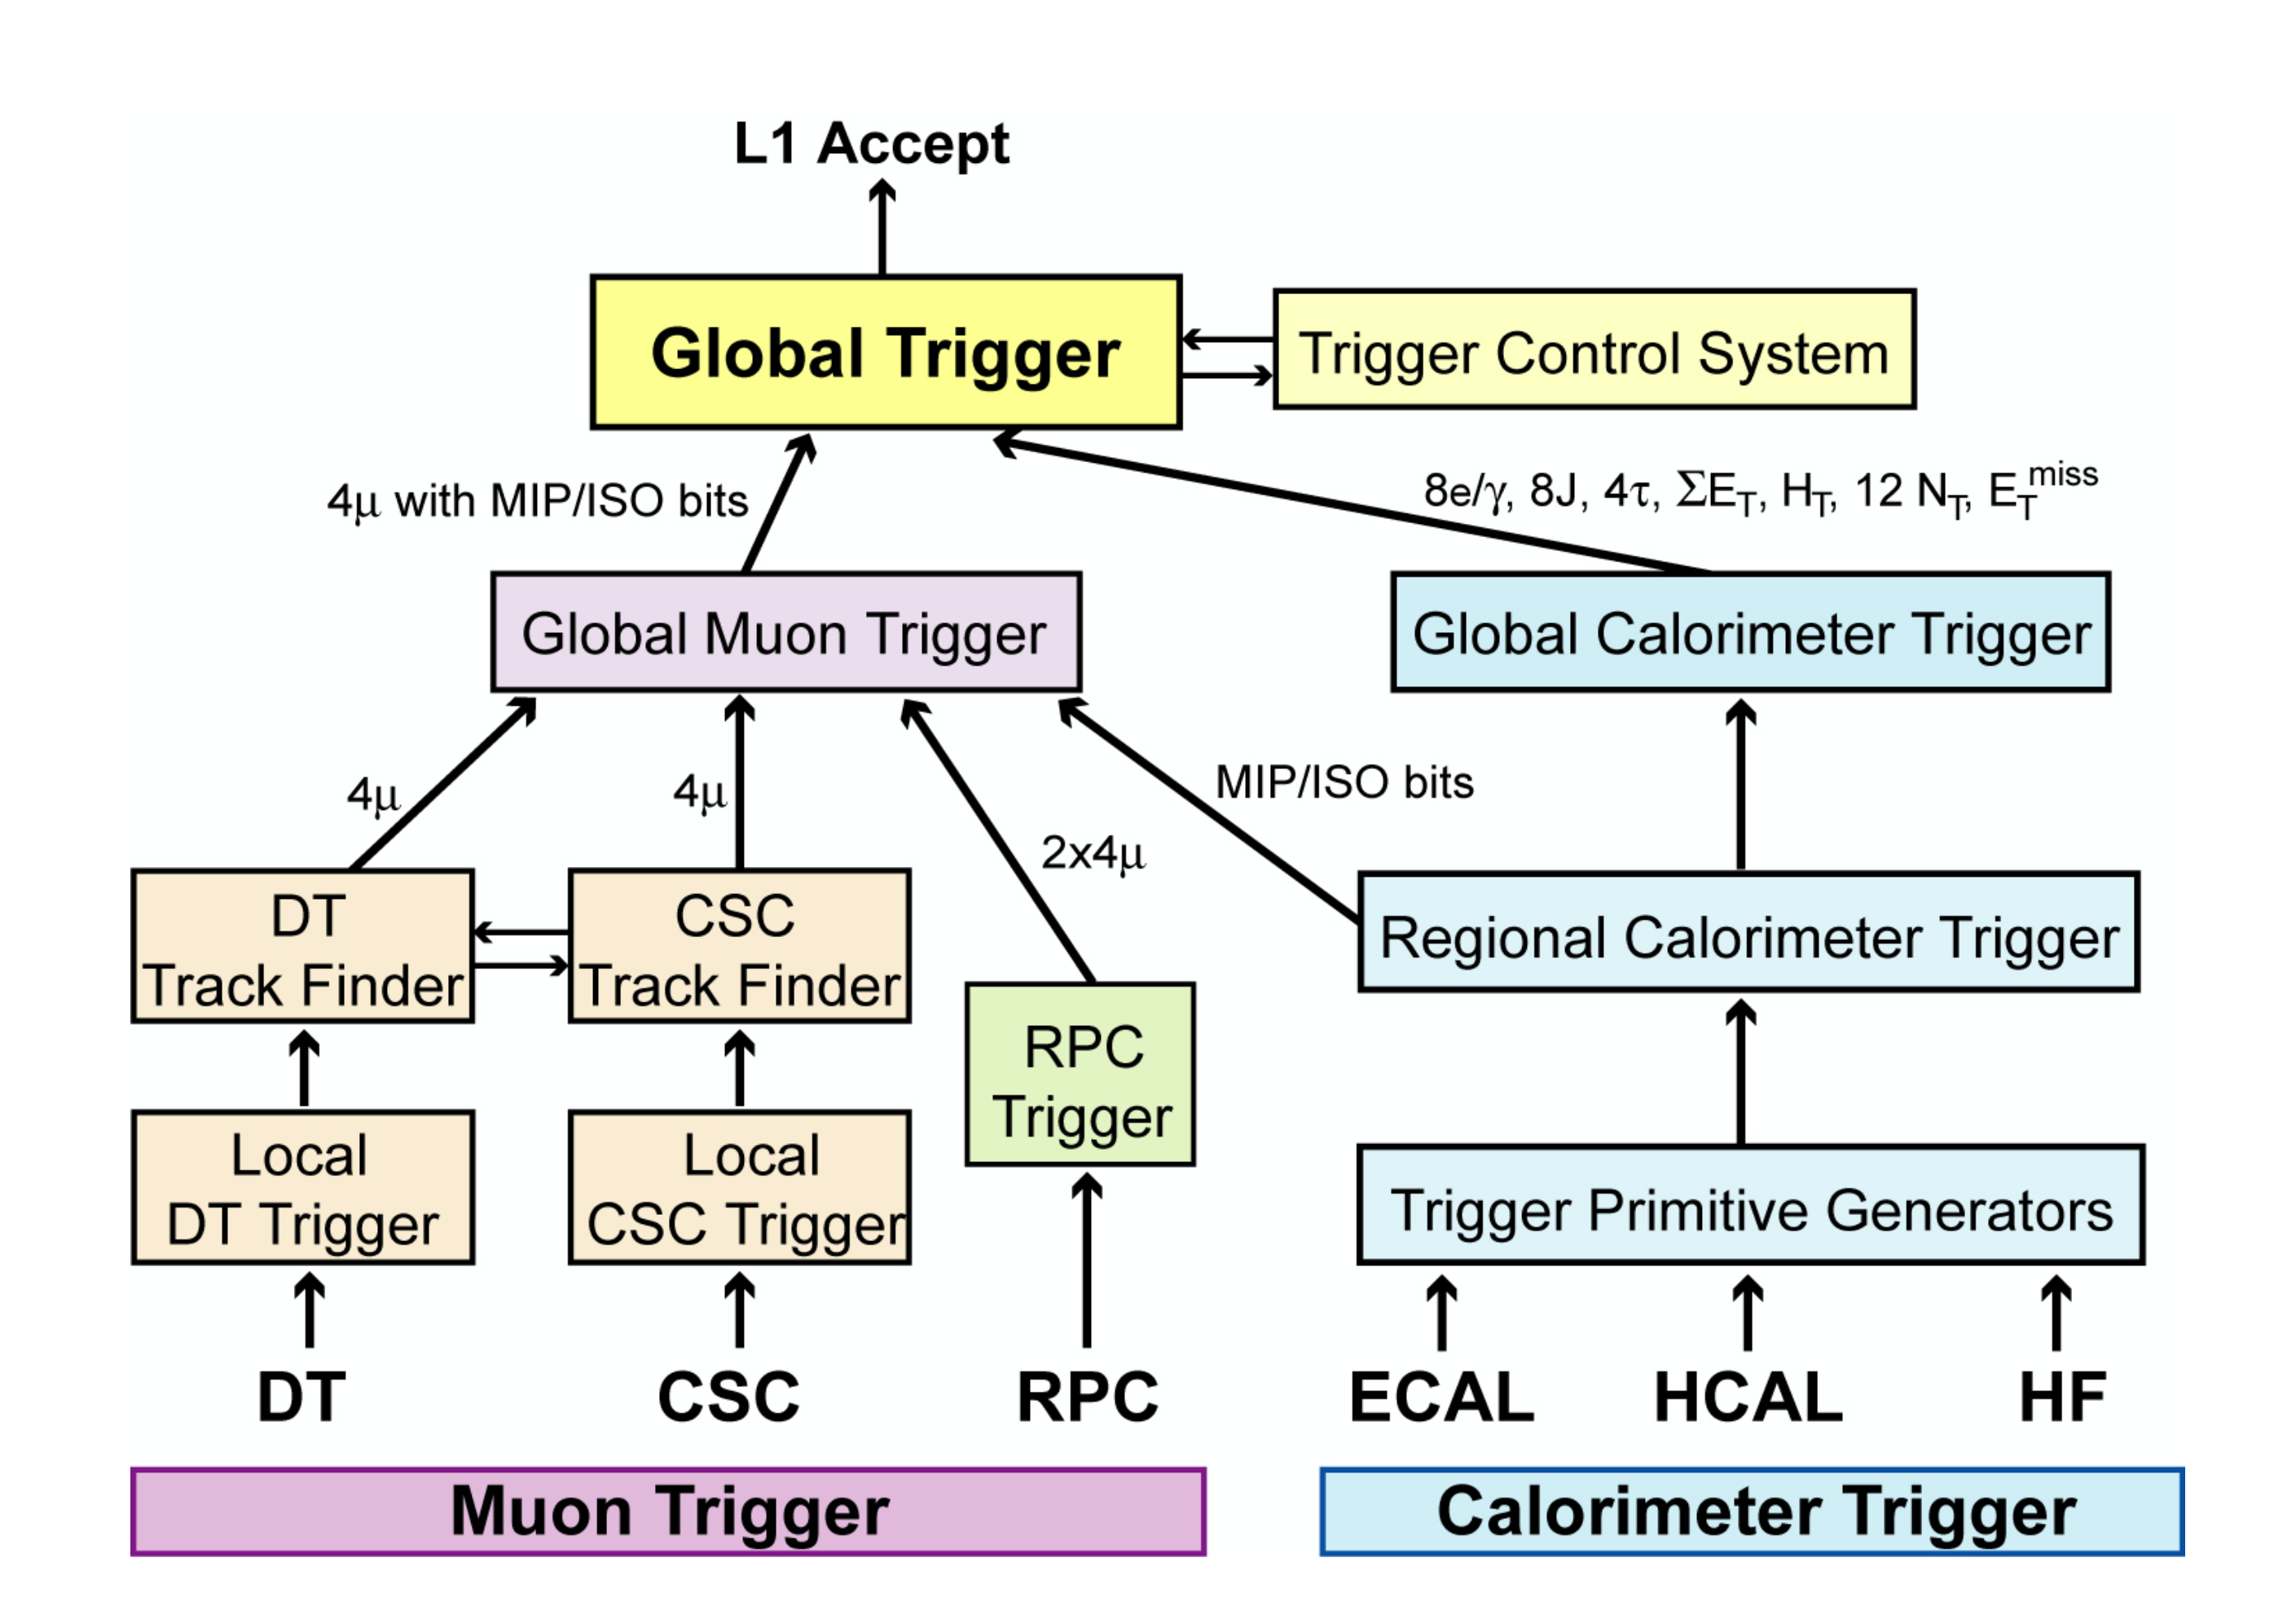
\includegraphics[width=\textwidth]{chapters/CMSExperiment/sectionTrigger/figures/trigger.png}
    \end{columns}
\end{frame}


\begin{frame}{CMS Detector}
    \begin{center}
        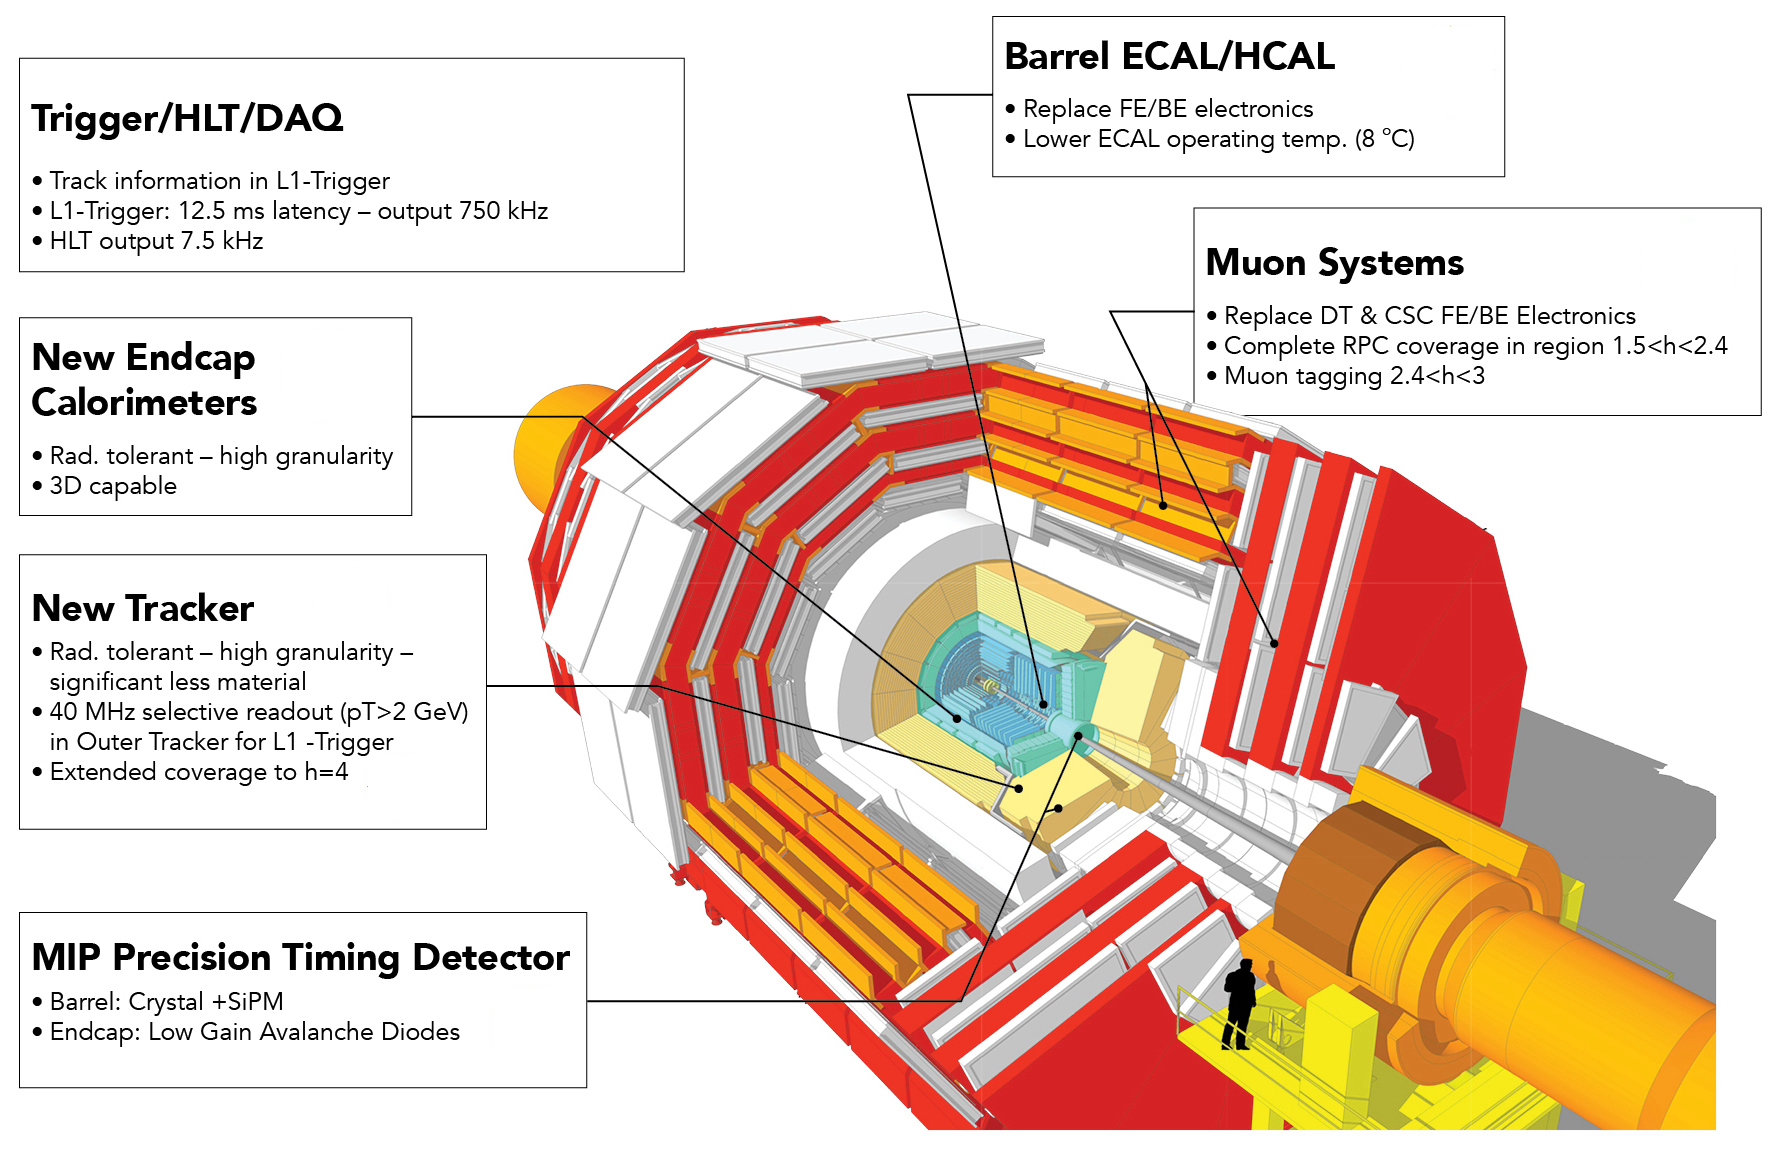
\includegraphics[width=0.9\textwidth]{slides/figures/CMS_NSF_DOE.jpeg}
    \end{center}
    \footnote{ https://www.classe.cornell.edu/NewsAndEvents/CLASSENewsCMS180129Ryan.html}
\end{frame}




\begin{frame}{Particle-Flow Reconstruction}
\smaller
    \begin{center}
        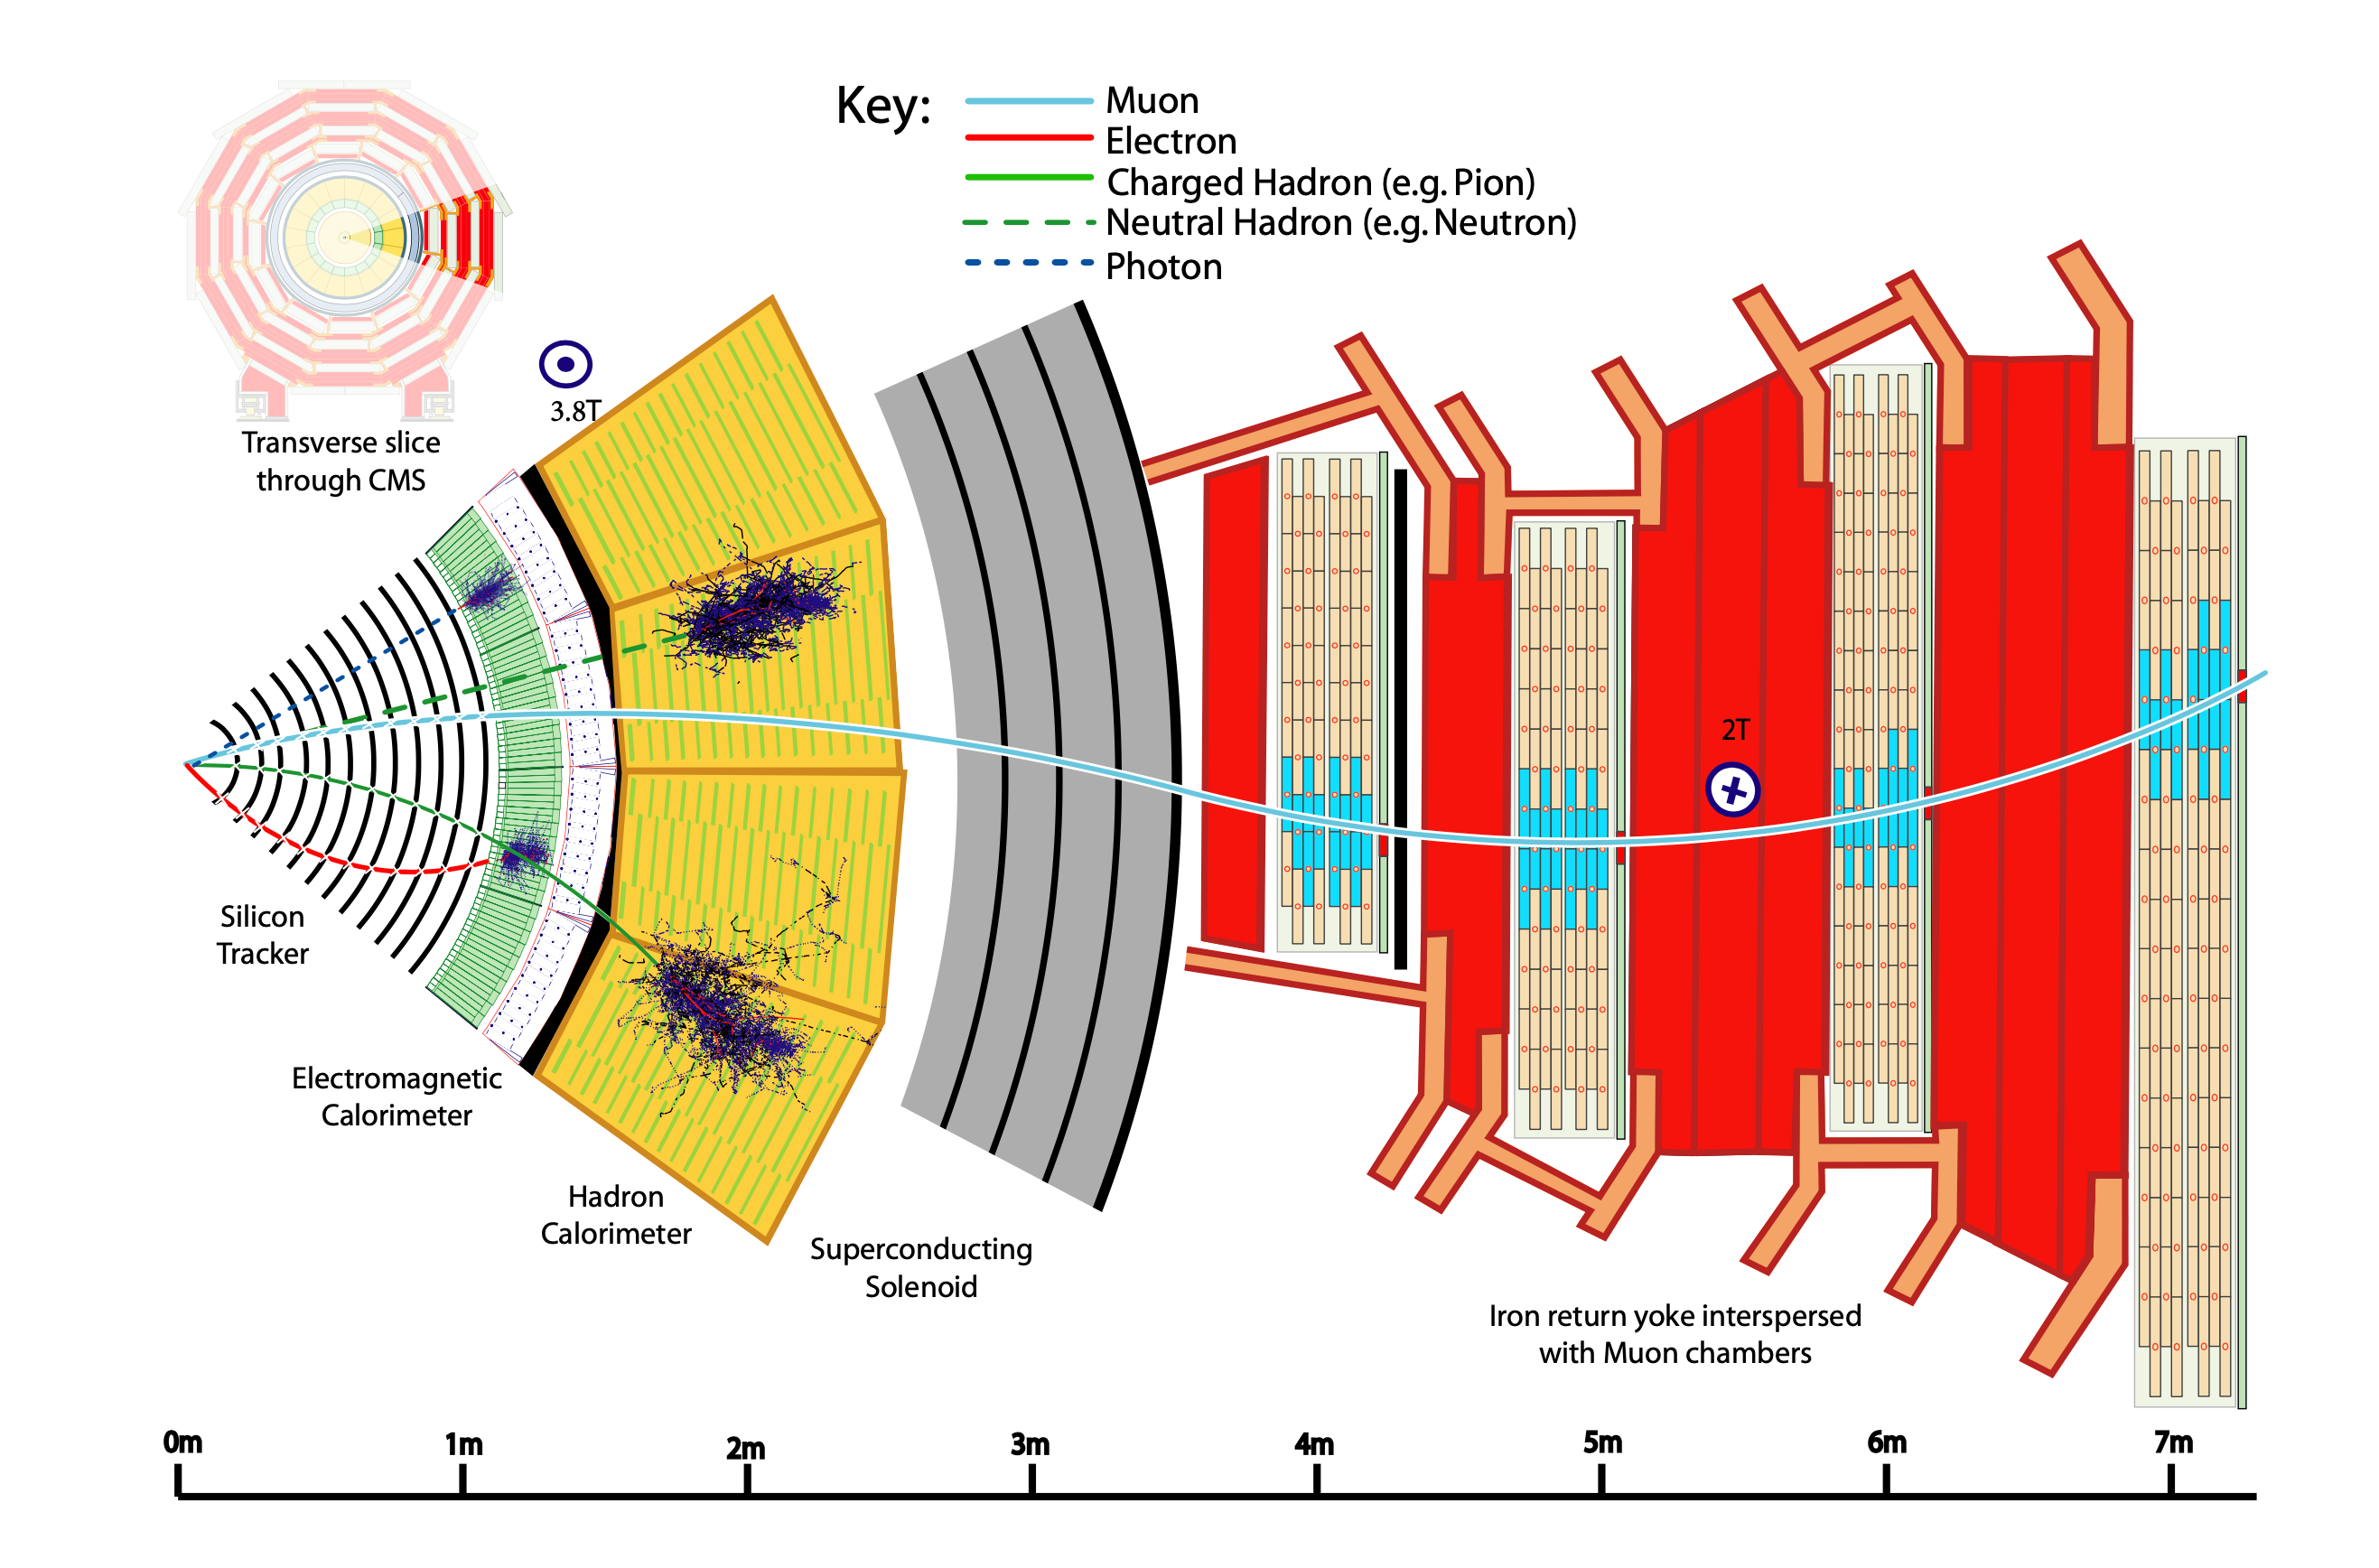
\includegraphics[width=0.7\textwidth]{chapters/CMSExperiment/sectionReconstruction/figures/pfa.png}
    \end{center}
    \begin{itemize} 
        \item combines information in all subdetector to construct final state particles (called PF candidate) muon, electron, charged hadron, neutral hadron, photon.
        \item main steps PF blocks, linking, identification/energy regression.
        \item Jets are clustered by anti-\kt based on PF candidates. 
    \end{itemize}
\end{frame}

\begin{frame}{Hadronic Tau Reconstruction}
\smaller
    \begin{center}
        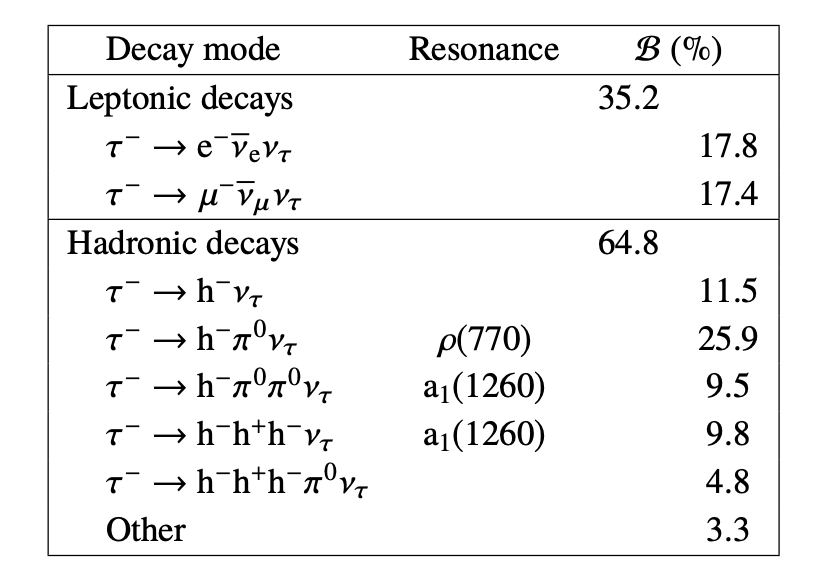
\includegraphics[width=0.5\textwidth]{slides/figures/tauDecay.png}
    \end{center}
    \begin{block}{Tau Property}
    \begin{itemize} 
        \item mass $m_\PGt = 1.776\GeV$ and lifetime $c\Gamma = 87\mum$
        \item 65\% decay hadronically
        \item fixed pattern of final-state particles
        \item defined visible mass at $\rho (770)$ and $a_1(1260)$
    \end{itemize}  
    \end{block}
\end{frame}

\begin{frame}{}
\smaller
    \begin{center}
        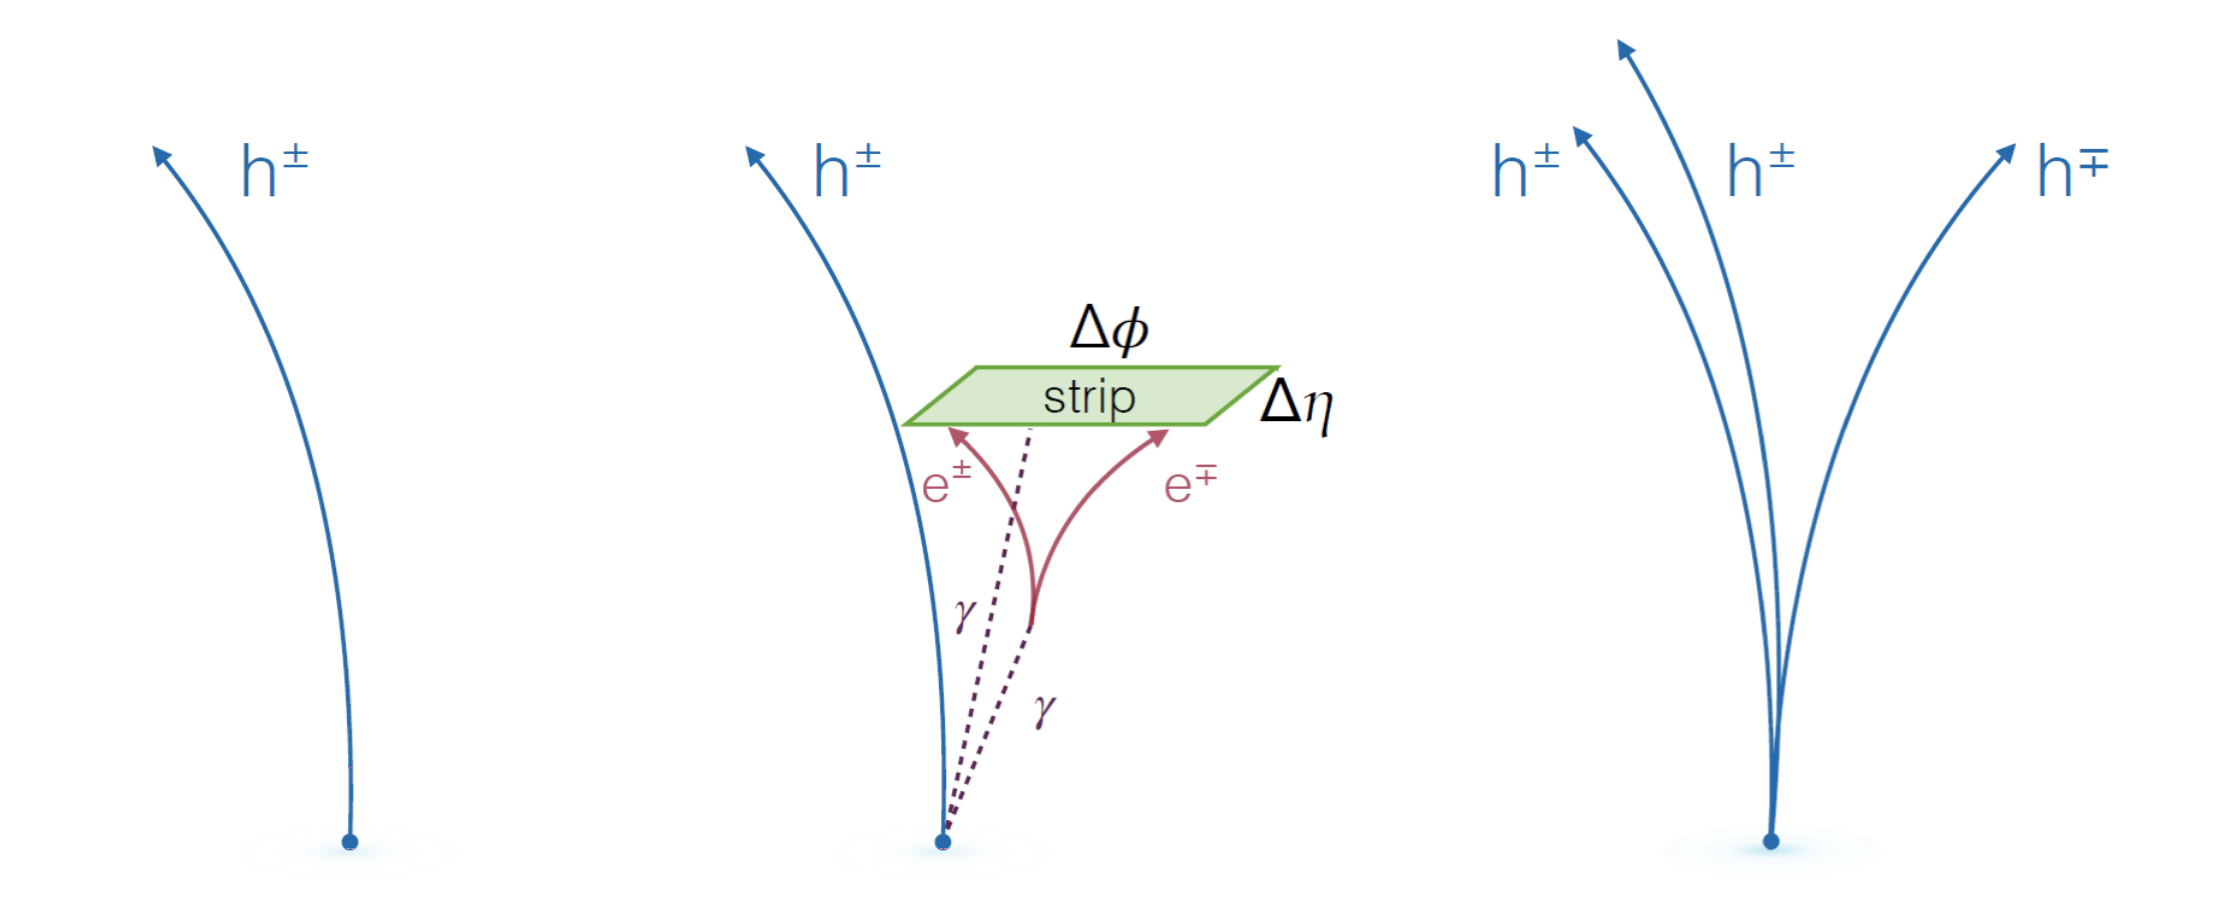
\includegraphics[width=0.6\textwidth]{slides/figures/tauReco.png}
    \end{center}
    \begin{block}{Hadrons-plus-strips (HPS)}
    Taus are reconstructed in their hadronic modes with Hadrons-plus-strips (HPS) algorithm from tagging PF jets
    \begin{itemize} 
        \item cluster \Pe/\PGg into strips. merging \Pe/\PGg in \pt decreasing order with a dynamic window size $\Delta\eta \times \Delta \phi = 0.20\pt^{-0.66} \times 0.35 \pt^{-0.71}$ 
        \item select charged hadrons (prong) $\pt>0.5\GeV$ and $d_{xy}<0.1$~cm.
        \item match to combination of hadrons and strips to \PGth decay modes.
        \item veto when
        \begin{itemize} 
        \smaller
            \item visible mass not competent with expected $\rho (770)$ and $a_1(1260)$ resonance
            \item not single charged
            \item any component falls outside signal cone $\Delta R_{sig} = \frac{3.0 \text{ GeV } } { \pt (\text{ hadronic system})  }$, with $0.05 \leq \Delta R_{sig} \leq 0.1.$
        \end{itemize}
    \end{itemize}  
    \end{block}
\end{frame}


\begin{frame}{Hadronic Tau Reconstruction}
\smaller
    
    \begin{columns}[c]
        \column{0.6\textwidth}
        \begin{block}{Discriminate against contamination}
        \begin{itemize} 
            \item discriminate against quark and gluon jets.
            \item iso-based discriminator: 
            \begin{itemize} 
            \smaller
                \item isolation is calculated energy sum in the ring between signal cone and $\Delta R = 0.3$ cone.
                \item quark and gluon jets tend to have larger isolation, while tau jets tend to have smaller.
            \end{itemize}
        
             
            % \begin{equation}
            % \tiny
            %     I_{\PGth} = \sum \pt^{\text{charged}} (d_z<0.2 \text{cm}) + \max \bigg( 0, \sum \pt^ \PGg - \Delta \beta \sum \pt^{\text{charged}} (d_z>0.2 \text{cm})  \bigg )
            % \end{equation}
            
            \item MVA-based discriminator: 
            \begin{itemize} 
            \smaller
                \item combine isolation and other variables sensitives to tau lifetime (e.g. SIP3D, d0).
                \item use boosted decision tree (BDT)
            \end{itemize}
        \end{itemize}
        \end{block}

        \column{0.4\textwidth}
        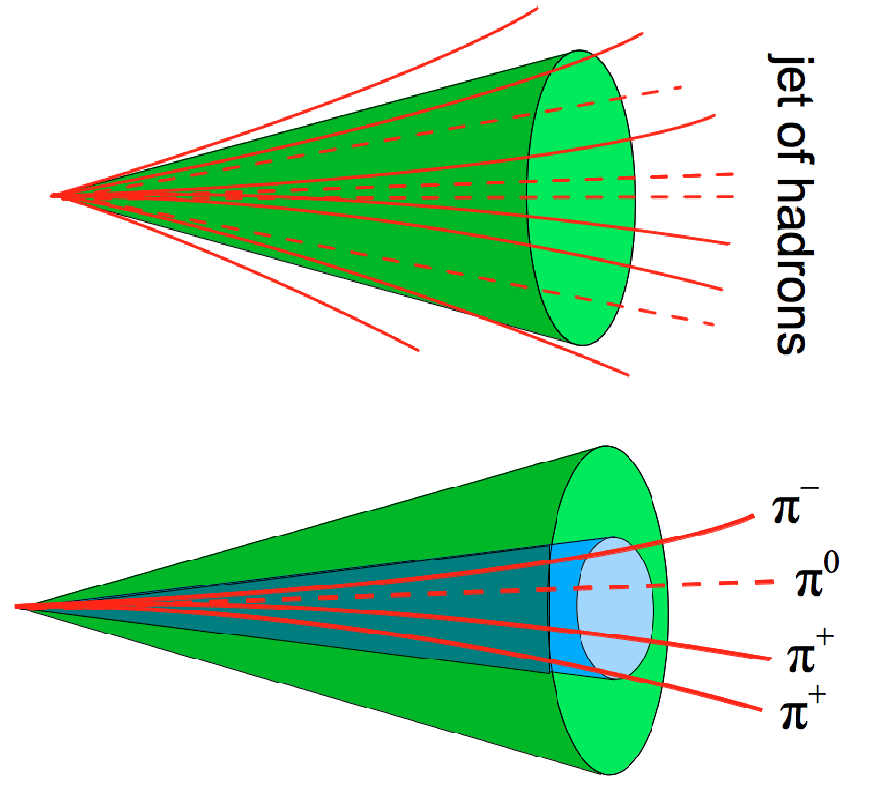
\includegraphics[width=\textwidth]{slides/figures/tausignature_trans.png}
    \end{columns}
    
\end{frame}
% \section{Measurement of WBr}

\subsection{Data and simulations}

\subsection{Selections}

\subsection{Calibrations and corrections}

\subsection{Modeling of background}

\subsection{Analysis methods}

\subsection{Systematics}

\subsection{Results}

% \section{Conclusion}

\begin{frame}{Conclusion}
\smaller
    \begin{itemize}
        \item For decades, LEP's result is the most precise and only \BWl measurement, showing $2.6\sigma$ tension with SM LU.

        \item We provide a new measurement with CMS using LHC 13\TeV collisions. Three individual leptonic branching fractions are measured simultaneous.
        \begin{itemize}
        \smaller
            \item  shape: \BWemt = 10.83(10)\%, 10.94(08)\%,10.77(21)\%
            \item  counting: \BWemt = 11.15(27)\%, 11.13(22)\%,10.63(65)\%
        \end{itemize}
        \item Counting analysis is limited by the tau identification systematics.
        \item Shape analysis is the currently the most precise measurement. 
        \begin{itemize}
        \smaller
            \item use \pt distribution to discriminate $\PW\to\PGtl$ and $\PW \to \ell$
            \item use extended data regions to constrain the tau related systematics.  
        \end{itemize}
        \item Two analysis are consist. SM LU is agreed.
        
        \item Assuming partial LU, $R^{\PW}_{\PGt/(\Pe,\PGm)} = 1.002(19)$ 
        \item Assuming fully LU, $\BWl=10.89(08)\%$ and $\BWh= 67.32(23)\%$, with which three SM quantities are derived
        \begin{itemize}
        \smaller
            \item \alpS = 0.094(33),  \sumCKM = 1.991(19), \absVcs = 0.969(11)
        \end{itemize}
    \end{itemize}
\end{frame}


\begin{frame}[allowframebreaks]
    \tiny{
    \bibliographystyle{unsrt}
    \bibliography{
        chapters/Introduction/chapterReference,
        chapters/Physics/chapterReference,
        chapters/CMSExperiment/chapterReference,
        chapters/Analysis/chapterReference,
        chapters/HGCal/chapterReference
        }
    }
\end{frame}


\end{document}
